\begin{figure}[h]
    \centering
    \begin{subfigure}[b]{0.23\textwidth}
        \centering
        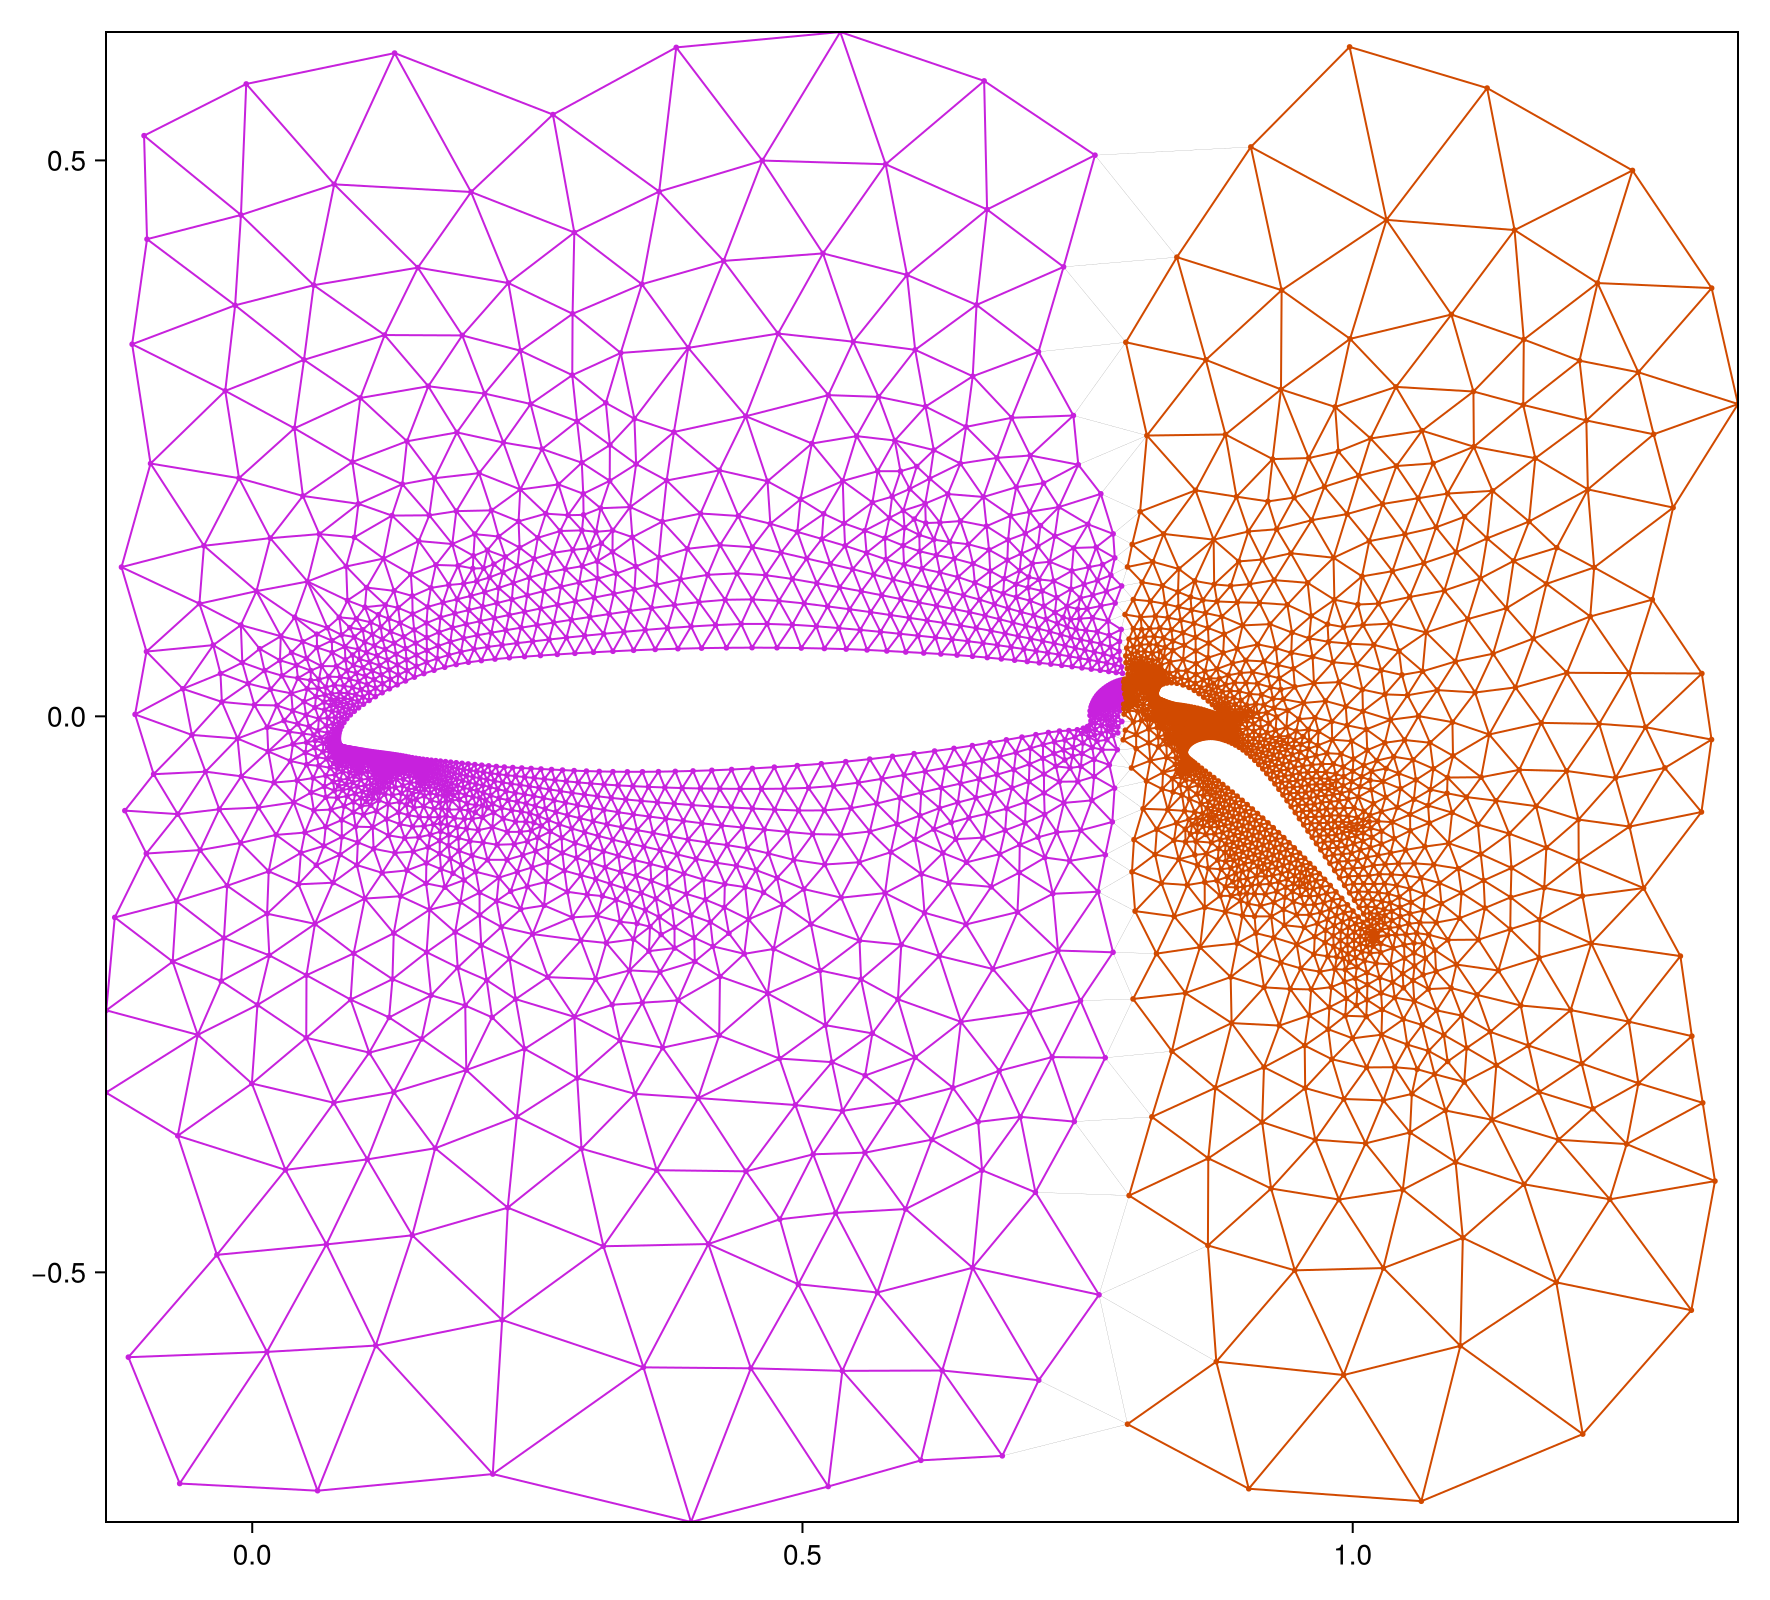
\includegraphics[width=\textwidth,  trim={100pt 74pt 0 0}, clip]{images/ex1_airfoil1_coordinate.png}
        \caption{Coordinate bisection}
        \label{fig:ex1_coord}
    \end{subfigure}
    \hfill
    \begin{subfigure}[b]{0.23\textwidth}
        \centering
        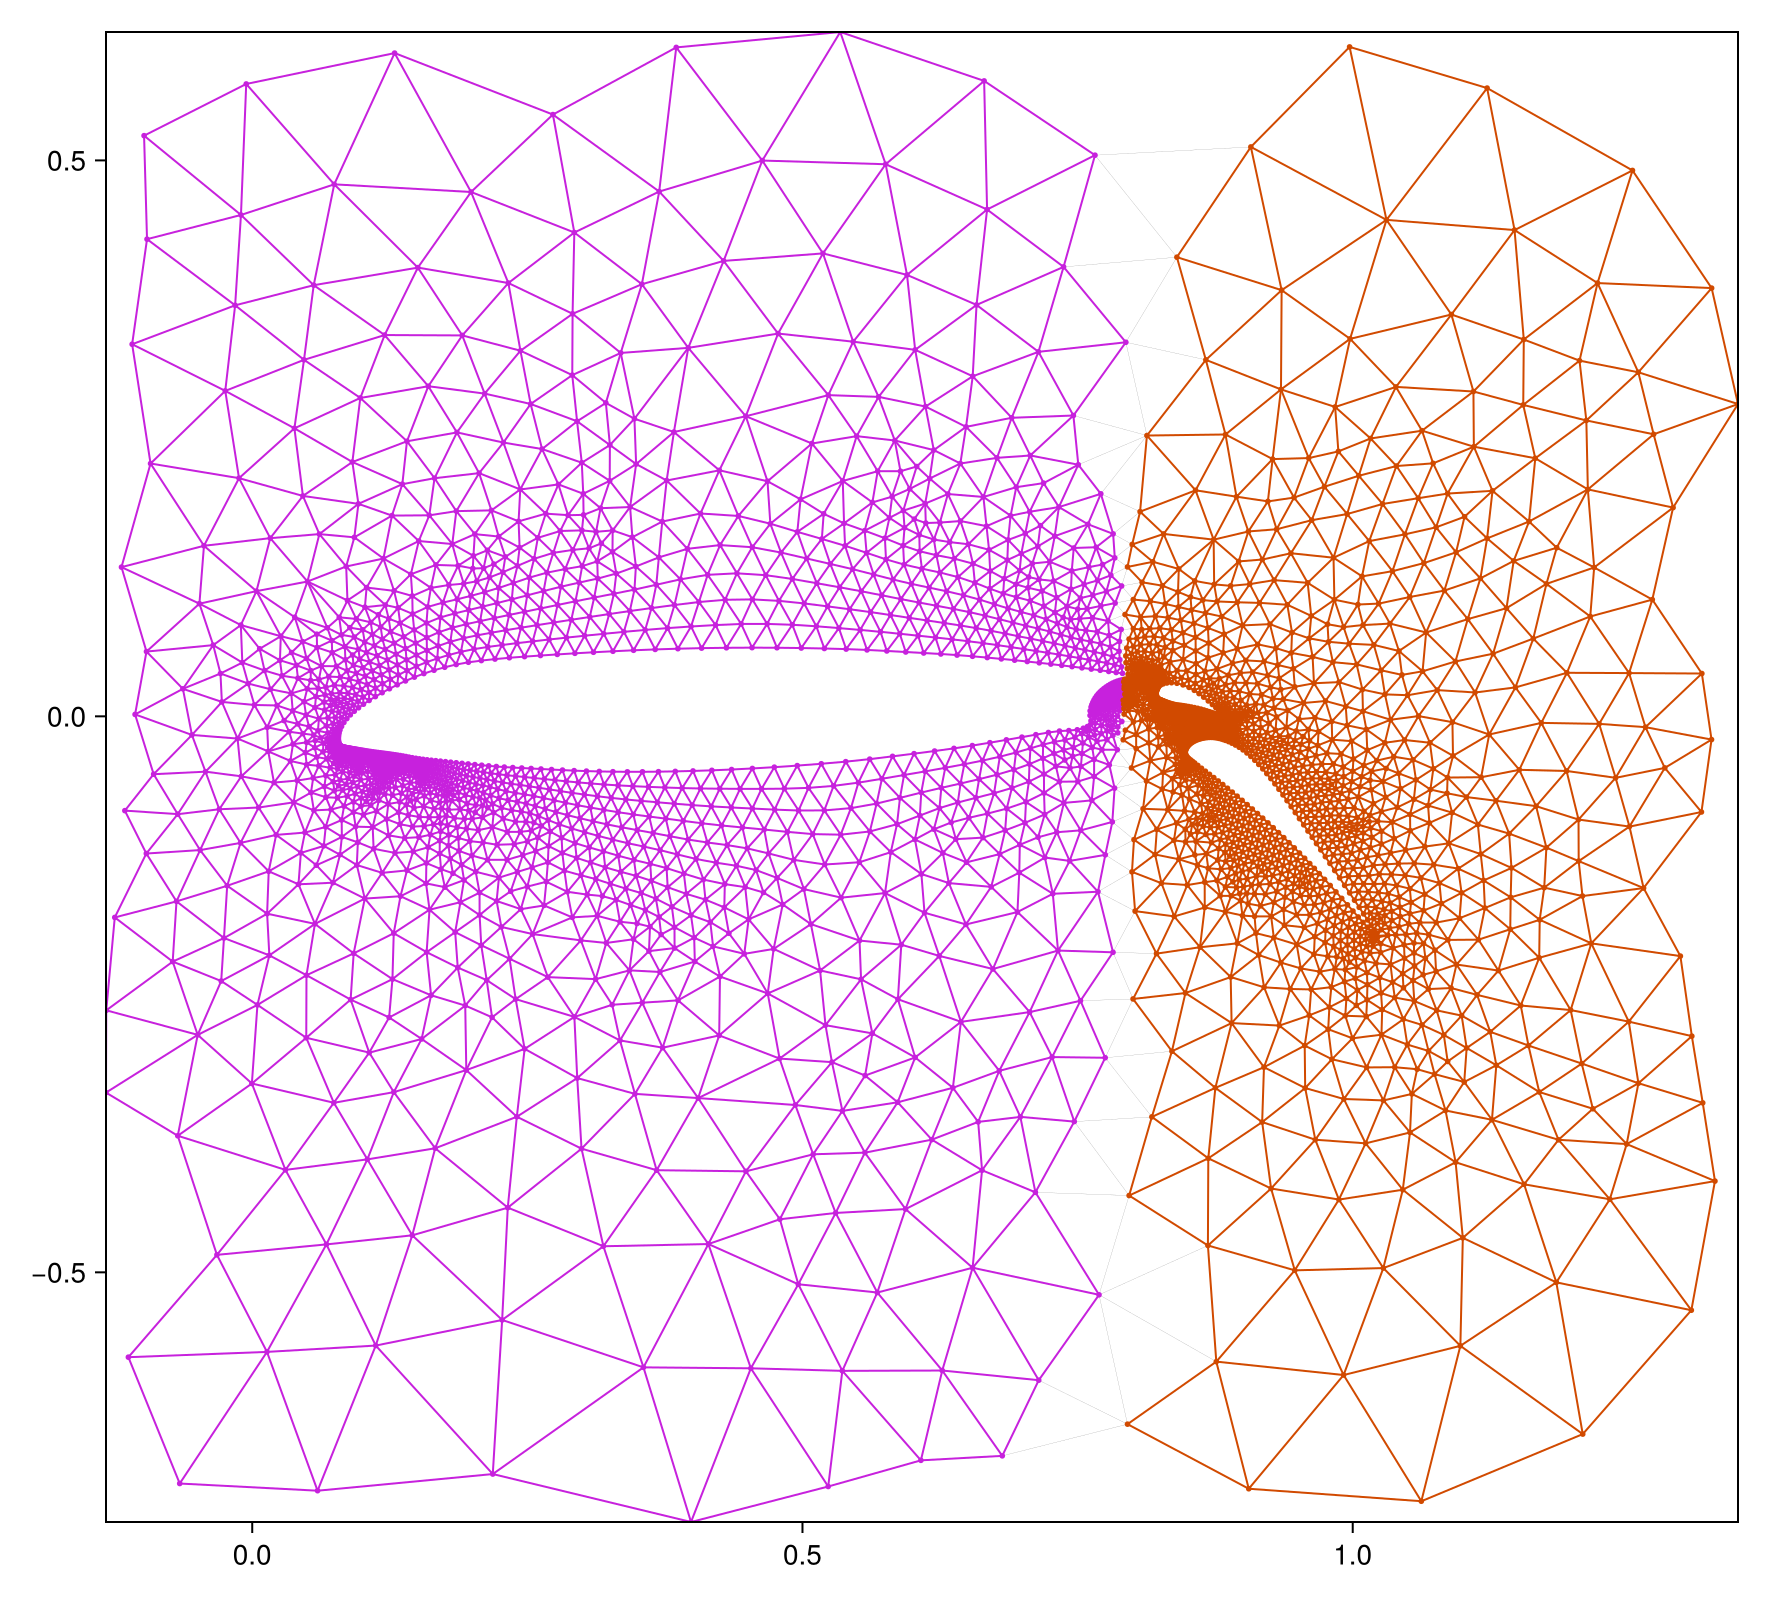
\includegraphics[width=\textwidth,  trim={100pt 74pt 0 0}, clip]{images/ex1_airfoil1_inertial.png}
        \caption{Inertial bisection}
        \label{fig:ex1_inertial}
    \end{subfigure}

    \vskip\baselineskip  % Adds vertical space between the rows

    \begin{subfigure}[b]{0.23\textwidth}
        \centering
        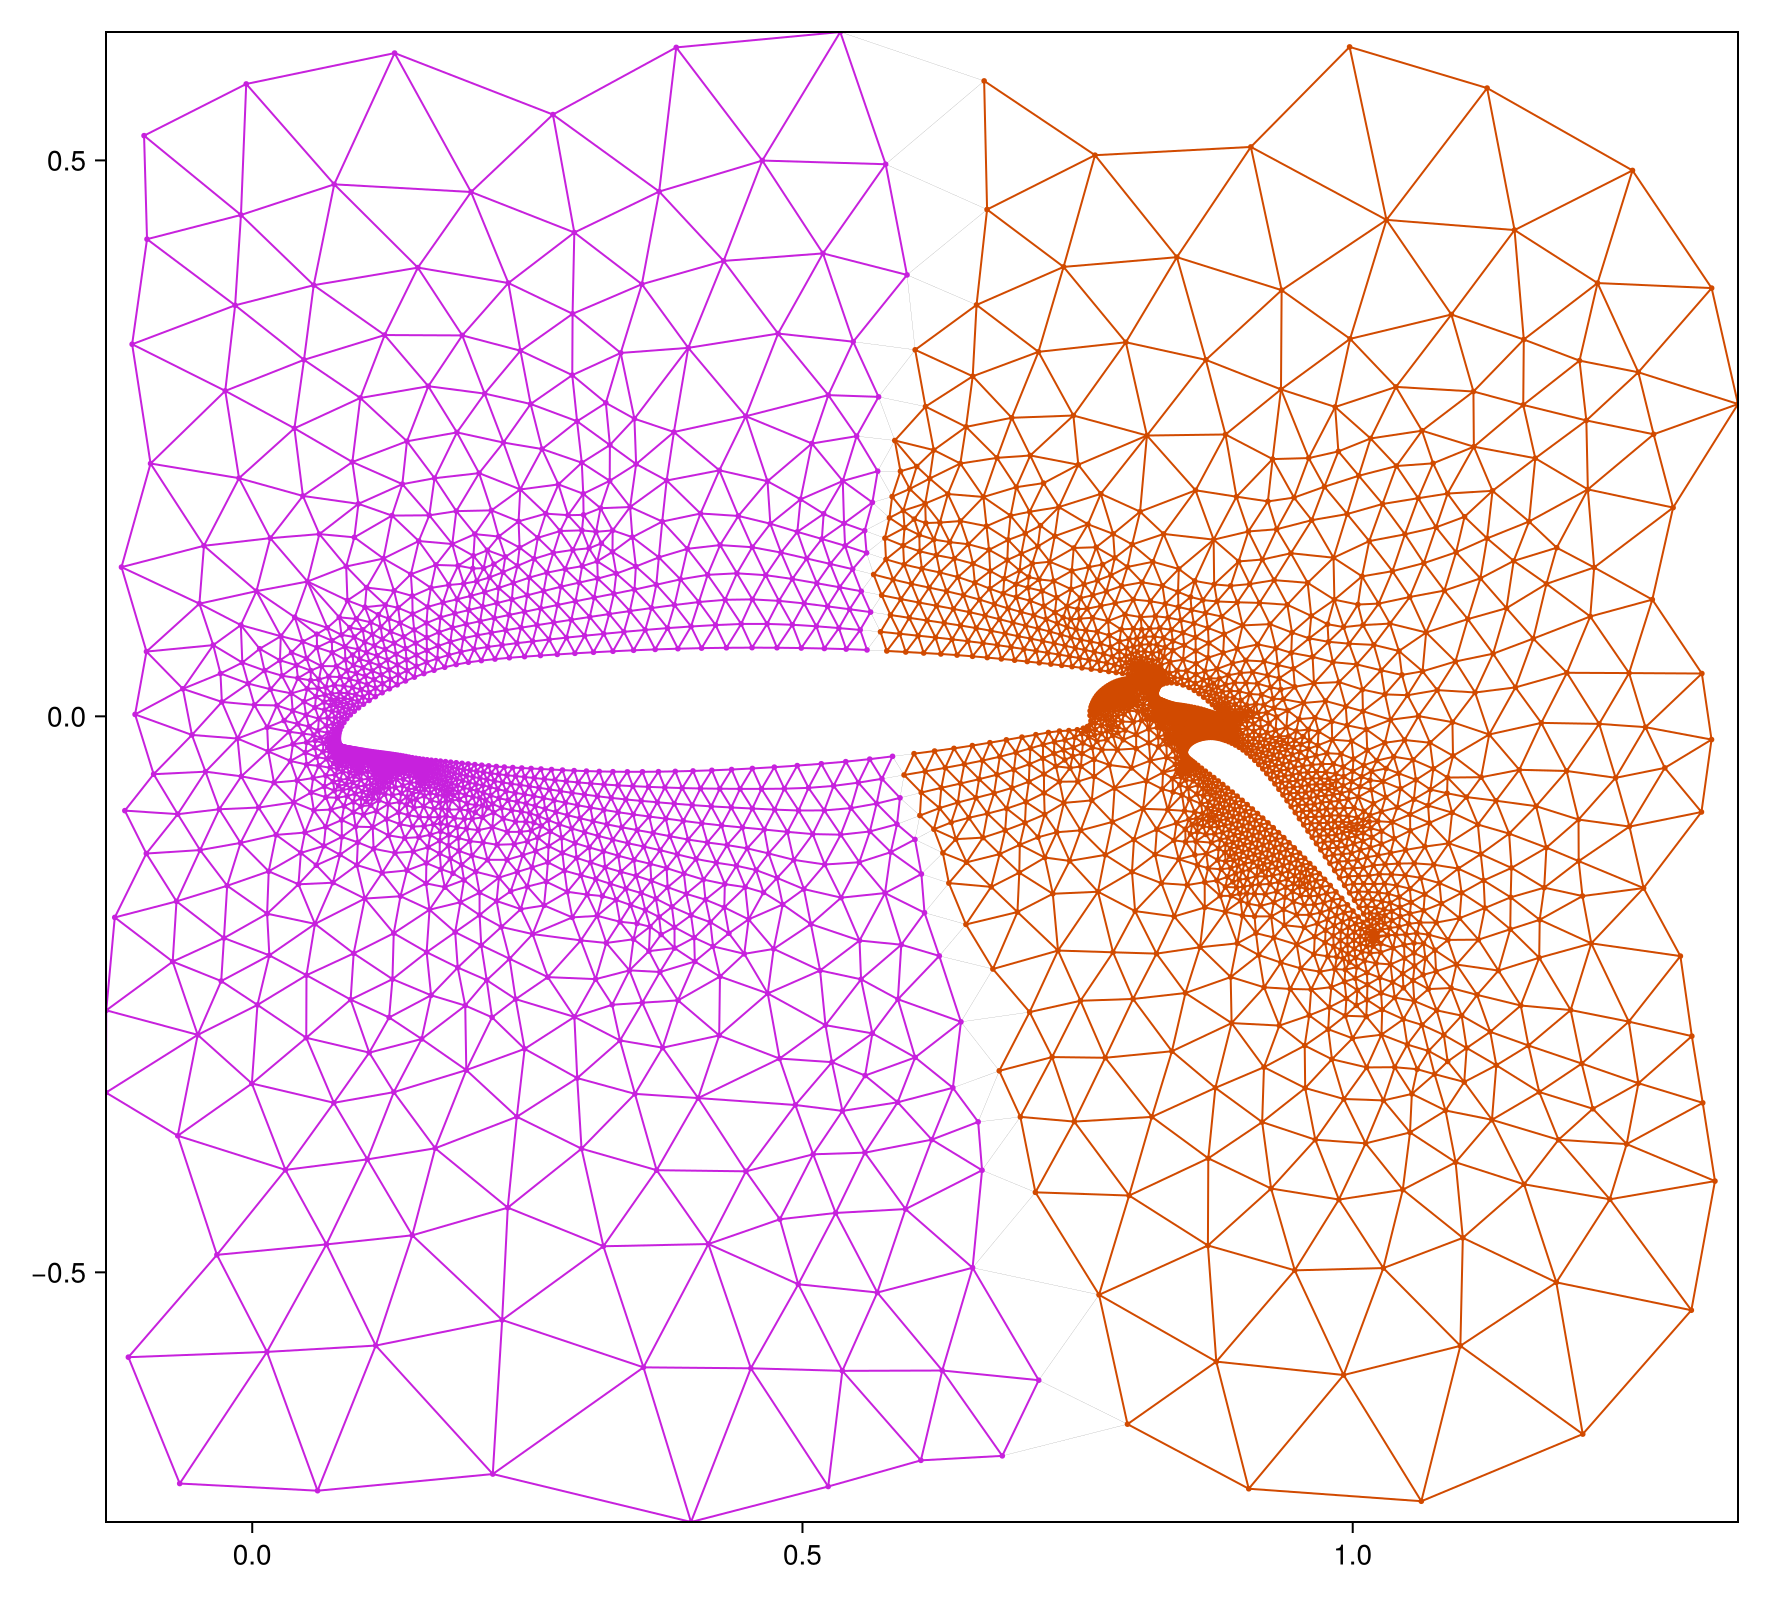
\includegraphics[width=\textwidth,  trim={100pt 74pt 0 0}, clip]{images/ex1_airfoil1_spectral.png}
        \caption{Spectral bisection}
        \label{fig:ex1_spectral}
    \end{subfigure}
    \hfill
    \begin{subfigure}[b]{0.23\textwidth}
        \centering
        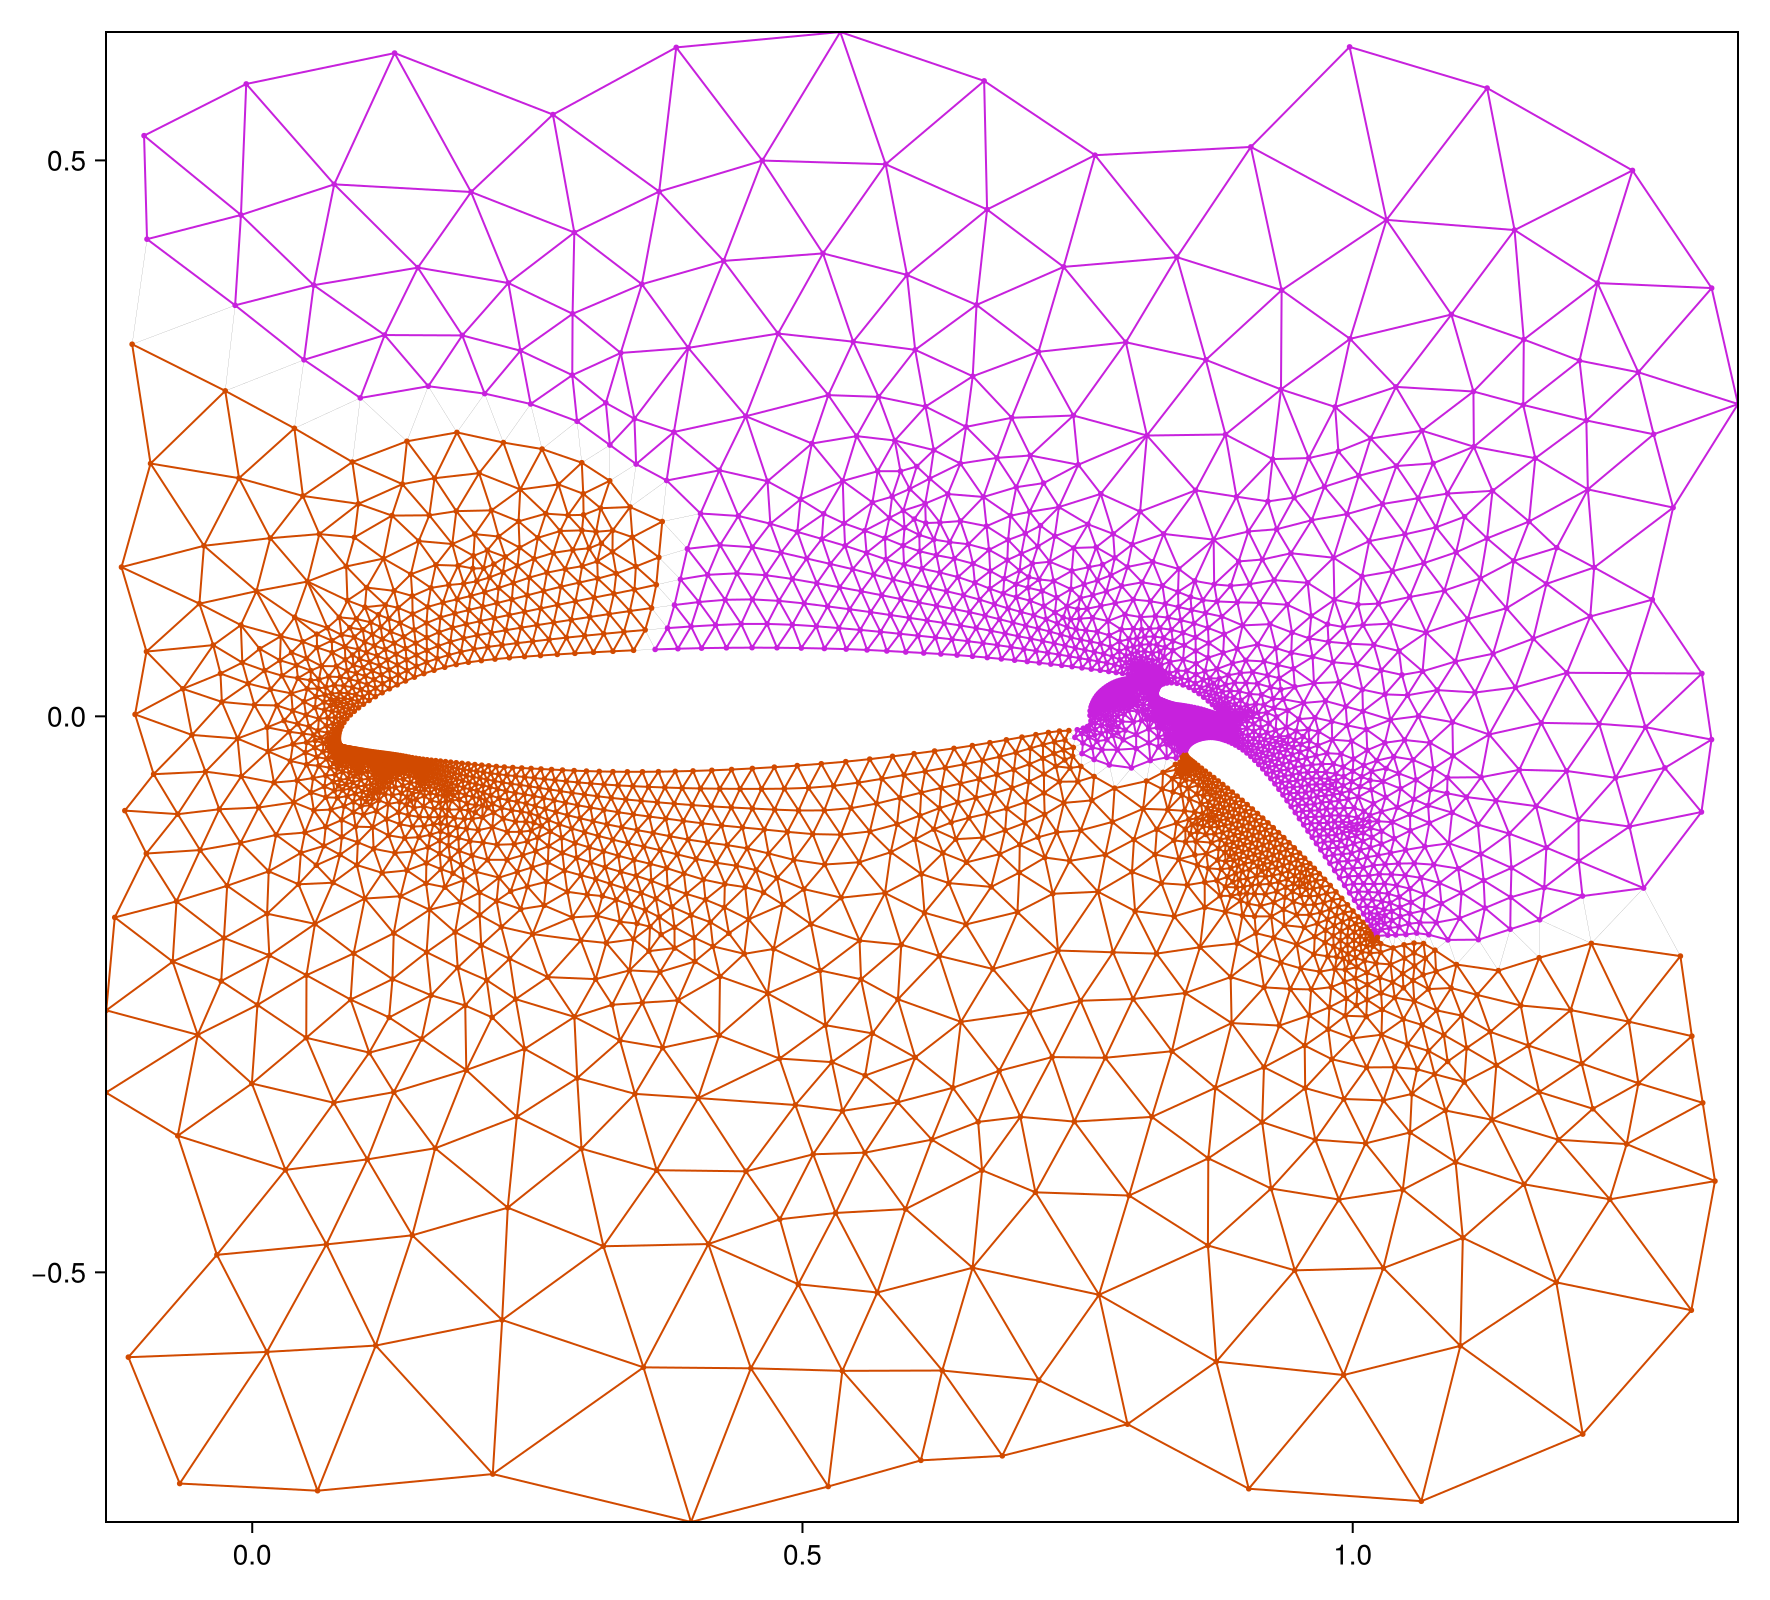
\includegraphics[width=\textwidth,  trim={100pt 74pt 0 0}, clip]{images/ex1_airfoil1_metis.png}
        \caption{Bisection using \texttt{METIS}}
        \label{fig:ex1_metis}
    \end{subfigure}

    \caption{Visualization of four graph bisection methods applied to the \texttt{airfoil1} mesh (4253 nodes and 12289 edges), illustrating differences in partitioning structure and edge cuts.}
    \label{fig:ex1_results}
\end{figure}
